\documentclass{article}
\usepackage{graphicx}
\usepackage{amsmath}
\usepackage{fancyhdr}
\usepackage{caption}

\pagestyle{fancy}
\rhead{K. Lin, K. Brendon, J. Klotz}
\lhead{Sfwr Eng 2AA4/Comp Sci 2ME3}
\cfoot{\thepage}

\title{Assignment 1}
\author{Kelvin Lin, Kerala Brendon, Jeremy Klotz\\Student Number: 001401464, 001424625, 001426853\\Course Code: SFWR ENG 2AA4/Comp Sci 2ME3}
\date{February 22\textsuperscript{nd}, 2016}

\begin{document}

\begin{titlepage}
\pagenumbering{gobble}
\maketitle
\center By virtue of submitting this document we electronically sign and date that the work being submitted is our own individual work.
\end{titlepage}

\tableofcontents
\newpage

\pagenumbering{arabic}
\section{Introduction and Architecture}
This report will document the design and the decisions made in Assignment 1 for Sfwr Eng 2AA4/Comp Sci 2ME3. The report will begin with an overview of the architecture and modules used in the application. Then the decomposition hierarchy will be examined in order to highlight its dependencies and to prepare a premise for a discussion on anticipated changes and other traditional software engineering practices. This report will end with a test plan, which will show that the application does fulfil the requirements up to the level specified in the document.

The architecture chosen for this application is the Model-Controller-View (MCV) architecture. The MCV architecture was chosen because it accentuates the principle of separation of concerns. The MCV architecture consists of three main components: the model, the controller, and the view. With the MCV architecture, the model represents data related to the logic the user works with, the view represents the user interface, and the controller facilitates the interaction between the model and the view. We believe that by using this architecture, different aspects of the program could be separated in order to facilitate testing and implementing future changes.

\section{Modular Decomposition and Hierarchy}
The application was designed using a top down approach. The top down approach was used in order to facilitate modular design and to accentuate separations of concerns. By using top down design, the application can be decomposed into modules, which are responsible for a single work assignment. Knowing the individual modules will allow programmers to program using the bottom-up approach, which would allow for early testing, and quick implementation of the application.

\newpage
The figure below shows the modular decomposition hierarchy for the application. Arrows point towards increasing modularity (from less modular to more modular):


\begin{minipage}{\linewidth}
\makebox[\linewidth]{
  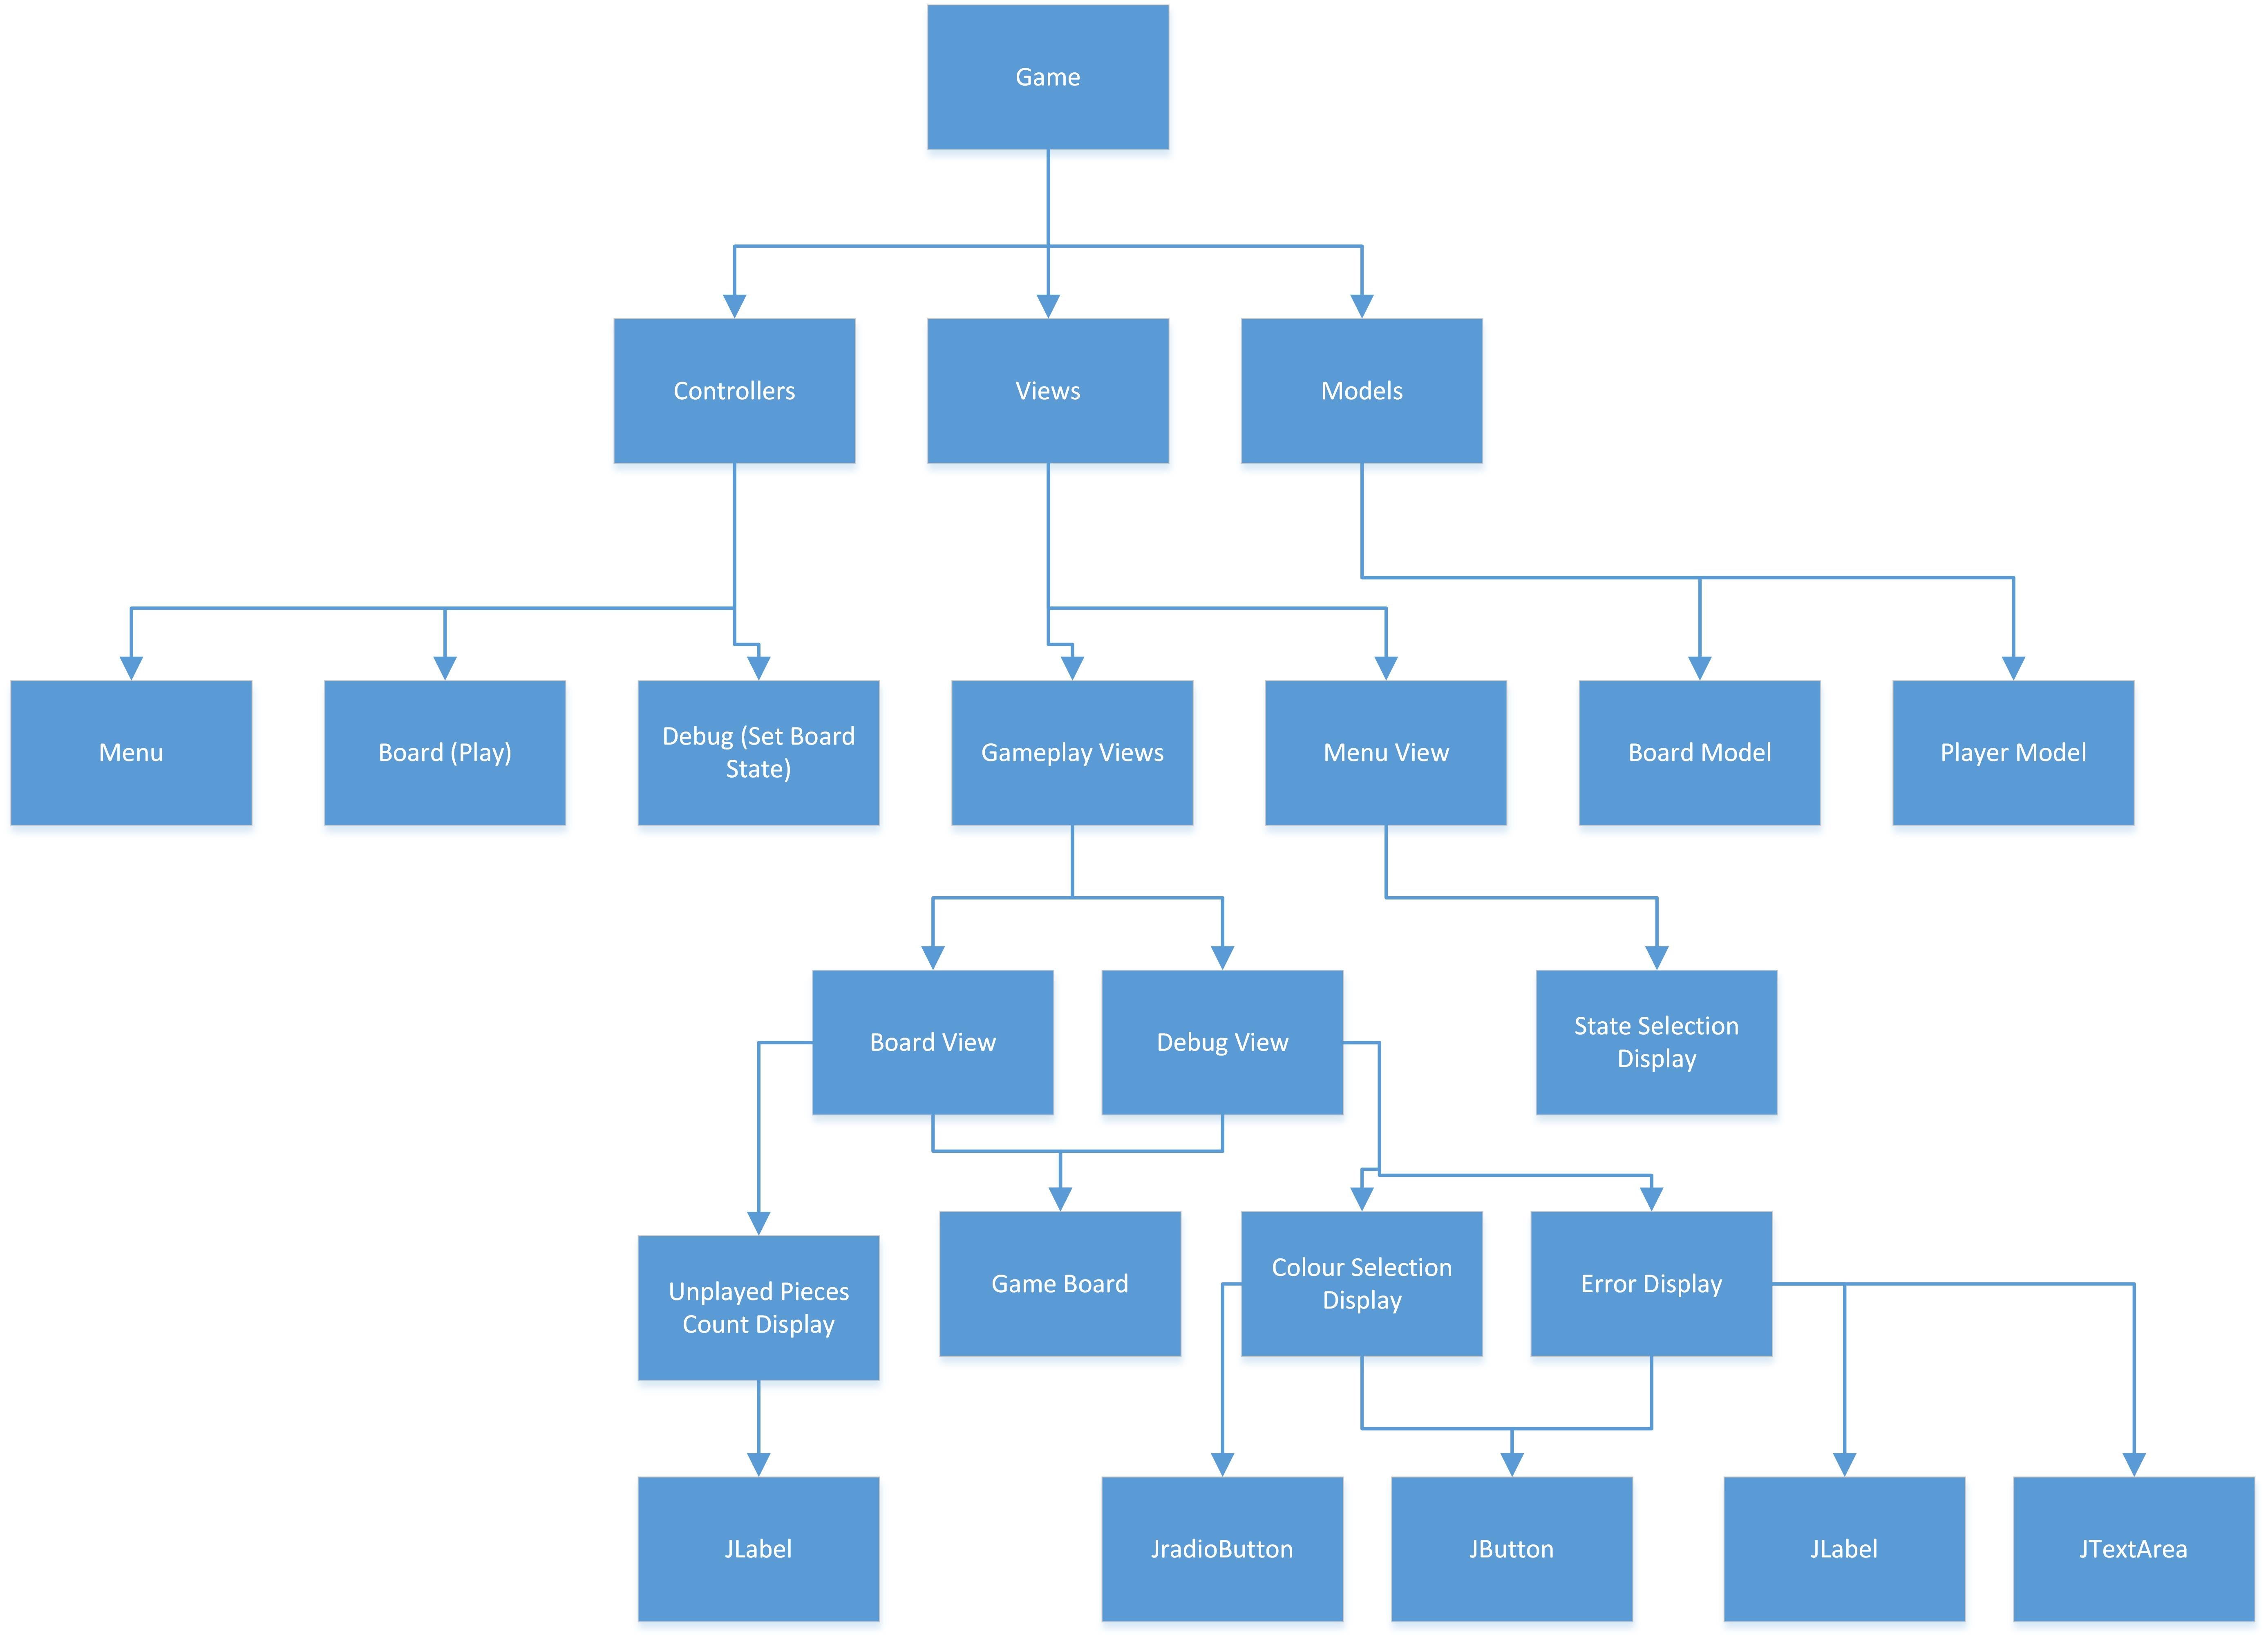
\includegraphics[keepaspectratio=true,scale=0.7]{Decomposition_Tree.jpg}}
  \captionof{figure}{The Decomposition Hierarchy}
\end{minipage}

\newpage
\section{Module Guide}

\subsection{MIS}

{}

{\textbf{CLASS: CIRCLE}}

{Defines a mathematical representation of a circle using its center
point and radius. Contains access programs to field variables, and to
detect user input.}

{}


{\textbf{INTERFACE}}


{\textbf{USES}}

{~~~~~~~~Point}

{\textbf{TYPE}}

{~~~~~~~~None}

{\textbf{ACCESS PROGRAMS}}

{~~~~~~~~\textbf{Circle(Point center, double radius)}}

{~~~~~~~~Constructor method required to create object of type Circle with a radius and center point.}

{~~~~~~~~~~~~~~~~}

{\textbf{getIntDiameter(): int}}

{Returns the diameter }{d}{~of the circle as an integer, \(d=2r\)

{~~~~~~~~~~~~~~~~}

{\textbf{getIntPointX(): int}}

{Returns the x-coordinate of the center point as an integer.}

{~~~~~~~~~~~~~~~~}

{\textbf{getIntPointY(): int}}

{Returns the y-coordinate of the center point as an integer.}

{~~~~~~~~~~~~~~~~}

{\textbf{getIntRadius(): int}}

{~~~~~~~~Returns the radius of the circle as an integer.}

{~~~~~~~~~~~~~~~~}

{\textbf{isMouseOver(Point mouse): boolean}}

{~~~~~~~~Returns }{TRUE }{if mouse is pointing over the circle,
otherwise returns FALSE}

{~~~~~~~~~~~~~~~~}

{}

{\textbf{CLASS: DEBUGCONTROLLER}}

{Creates the window and all labels or buttons needed to access and
update the view which in turn will change values in the model.}

{}

{\textbf{INTERFACE}}

{}

{\textbf{USES}}

{~~~~~~~~BoardView}

{~~~~~~~~DebugController}

{\textbf{TYPE}}

{~~~~~~~~none}

{\textbf{ACCESS PROGRAMS}}

{~~~~~~~~\textbf{DebugController(int N)}}

{Construct the state based on the number of layers.}

{~~~~~~~~}

{}

{\textbf{CLASS: ERRORDIALOG}}

{Defines a dialog box to display error messages to the user. Contains an
access program to respond to the user's input.}

{}

{\textbf{INTERFACE}}

{\textbf{USES}}

{~~~~~~~~JDialog, ActionListener}

{TYPE}

{~~~~~~~~None}

{\textbf{ACCESS PROGRAMS}}

{~~~~~~~~\textbf{ErrorDialog(JFrame parent, String title, String message)}}

{Initializes a dialog to display any errors found during the execution
of the application}

{~~~~~~~~~~~~~~~~}

{\textbf{actionPerformed(ActionEvent e)}}

{~~~~~~~~Responds to the user's input}

{~~~~~~~~~~~~~~~~~~~~~~~~}

{~~~~~~~~}

{\textbf{CLASS: MENUCONTROLLER}}

{Defines a controller to mediate the views and models used in the menu.}

{}

{\textbf{INTERFACE}}

{\textbf{USES}}

{~~~~~~~~MenuView, JFrame}

{\textbf{TYPE}}

{~~~~~~~~None}

{\textbf{ACCESS PROGRAMS}}

{~~~~~~~~\textbf{MenuController()}}

{~~~~~~~~Instantiates the view and any field variables used in the
module.}

{~~~~~~~~~~~~~~~~}

{\textbf{run(): void}}

{~~~~~~~~Runs any operations associated with the controller.}

{~~~~~~~~~~~~~~~~}

{\textbf{getJFrame(): JFrame}}

{~~~~~~~~Returns the JFrame.}

{~~~~~~~~~~~~~~~~}

{}

{\textbf{CLASS: MENUVIEW}}

{Defines a view for the menu screen.}

{}

{\textbf{INTERFACE}}

{\textbf{USES}}

{~~~~~~~~Screen}

{\textbf{TYPE}}

{~~~~~~~~None}

{\textbf{ACCESS PROGRAMS}}

{~~~~~~~~\textbf{MenuView(int N)}}

{~~~~~~~~Instantiates the objects on the screen and any field variables
used in the module.}

{~~~~~~~~~~~~~~~~}

{\textbf{getState():int}}

{Returns the state of the application.}

{~~~~~~~~}

{\textbf{updateScreen(): void}}

{Updates the screen.}

{~~~~~~~~}

{\textbf{paintComponent(Graphics g): void}}

{Draws the required components onto the screen.}

{~~~~~~~~~~~~~~~~}

{~~~~~~~~}

{\textbf{CLASS: PLAYER}}

{Each player is determined by two integers. ~An integer that represents
their color , and the number of pieces they have left to place.}

{}

{\textbf{INTERFACE}}

{\textbf{USES}}

{~~~~~~~~None}

{\textbf{TYPE}}

{~~~~~~~~None}

{~~~~~~~~~~~~~~~~}

{~~~~~~~~\textbf{Player(int color, int numberOfUnplayedPieces)}}

{~~~~~~~~Initializes field variables}

{~~~~~~~~}

{\textbf{getColor():int}}

{~~~~~~~~Returns the color of the player.}

{~~~~~~~~~~~~~~~~}

{\textbf{getNumberOfUnplayedPieces():int}}

{~~~~~~~~Returns the number of pieces the player has yet to place.}

{~}

{\textbf{placePiece(): void}}

{~~~~~~~~Models the action of the user playing a piece on the board.}

{~~~~~~~~~~~~~~~~}

{\textbf{CLASS: POINT}}

{Defines a mathematical representation of a circle using its
x-coordinate and its y-coordinate.}

{}

{\textbf{INTERFACE}}

{\textbf{USES}}

{~~~~~~~~None}

{\textbf{TYPE}}

{~~~~~~~~None}

{\textbf{ACCESS PROGRAMS}}

{~~~~~~~~\textbf{Point(double x, double y)}}

{~~~~~~~~Initializes the field variables}

{~~~~~~~~~~~~~~~~}

{\textbf{getX(): double}}

{~~~~~~~~Returns the x-coordinate.}

{~~~~~~~~~~~~~~~~}

{\textbf{getY(): double}}

{Returns the y-coordinate.}

{~~~~~~~~~~~~~~~~}

{\textbf{getIntX(): int}}

{~~~~~~~~Returns the x-coordinate as an integer.}

{~~~~~~~~~~~~~~~~}

{\textbf{getIntY(): int}}

{~~~~~~~~Returns the y-coordinate as an integer.}

{~~~~~~~~~~~~~~~~}

{\textbf{getDistance(Point that): double}}

{~~~~~~~~Return the distance between two point objects, \(d=\sqrt{(x_{2} - x_{1})^{2} + (y_{2} - y_{1})^{2}}\)}

{~~~~~~~~}

{}

{\textbf{CLASS: RECTANGLE}}

{Defines a mathematical representation of a rectangle defined by the top
left, top right, and bottom left corners.}

{}

{\textbf{INTERFACE}}

{\textbf{USES}}

{~~~~~~~~Point}

{\textbf{TYPE}}

{~~~~~~~~None}

{\textbf{ACCESS PROGRAMS}}

{~~~~~~~~}{\textbf{Rectangle(Point topLeft, Point topRight, Point bottomRight)}}

{~~~~~~~~Initializes the field variables}

{~~~~~~~~}

{\textbf{getTopLeft(): Point}}

{~~~~~~~~Returns the top left point of the rectangle.}

{~~~~~~~~}

{\textbf{getTopRight(): Point}}

{Returns the top right point of the rectangle. }

{~~~~~~~~~~~~~~~~}

{\textbf{getBottomRight(): Point}}

{~~~~~~~~Returns the bottom right point of the rectangle.}

{~~~~~~~~~~~~~~~~}

{\textbf{getIntWidth(): int}}

{~~~~~~~~Returns the width of the rectangle, \(w = |x_{top left} - x_{top right}|\)}

{~~~~~~~~~~~~~~~~}

{\textbf{getIntHeight():int }}

{~~~~~~~~Return the height of the rectangle, \(h = |y_{top right} - y_{bottom right}|\)}

{~~~~~~~~~~~~~~~~}

{\textbf{getTopLeftIntX(): int}}

{~~~~~~~~Return the x-coordinate of the top left corner as an integer.}

{~~~~~~~~~~~~~~~~}

{\textbf{getTopLeftIntY(): int}}

{~~~~~~~~Return the y-coordinate of the top left corner as an integer.}

{~~~~~~~~~~~~~~~~}

{\textbf{getBottomLeft(): Point}}

{~~~~~~~~Return the bottom left point, defined by \((x_{top left}, y_{bottom right})\)}

{~~~~~~~~}

{\textbf{CLASS: SCREEN}}

{Declares a function that will be used in classes that extend from it.
In this assignment, that would be the classes ~menuView, and boardView.
It is a template for the views. }

{}

{\textbf{INTERFACE}}

{\textbf{USES}}

{~~~~~~~~None}

{\textbf{VARIABLES}}

{None}

{\textbf{ACCESS PROGRAMS}}

{\textbf{updateScreen():void}}

{~~~~~~~~Updates the screen}

{}

{\textbf{CLASS: VIEW}}

{What the user sees\ldots{}}

{\textbf{INTERFACE}}

{\textbf{USES}}

{~~~~~~~~Board}

{~~~~~~~~Circle}

{\textbf{TYPE}}

{~~~~~~~~None}

{\textbf{ACCESS PROGRAMS}}

{\textbf{View(int N)}}

{Constructor method of type View. Creates a board of the current
application state.}

{~~~~~~~~~~~~~~~~}

{\textbf{setBoardState(int number, int state): void}}

{Set the state of the board.}

{~~~~~~~~~~~~~~~~}

{\textbf{getBoardState(int number): int}}

{Return the current state of the board from accessing
getPieceState.}

{~~~~~~~~~~~~~~~~}

{\textbf{getCircles(): Circle{[}{]}}}

{Return the array of all circles in the board.}

{~~~~~~~~~~~~~~~~}

{\textbf{setStates(int{[}{]} states): void}}

{Set the states of the game.}

{~~~~~~~~~~~~~~~~}

{}

{\textbf{CLASS: BOARD}}

{This is an abstract representation of the game board. It keeps the
state of each piece in a 1 dimensional array in order to reduce run time
and space.}

{\textbf{INTERFACE}}

{\textbf{USES}}

{~~~~~~~~None}

{\textbf{TYPE}}

{~~~~~~~~None}

{\textbf{ACCESS PROGRAMS}}

{\textbf{Board(int N)}}

{Constructs an array representation of the board.}

{~}

{\textbf{Board(int N, int{[}{]} pieces)}}

{Constructs an array representation of the board given a preset state.}

{~}

{\textbf{setPieces(int{[}{]} pieces): void}}

{Initializes the pieces array.}

{~}

{\textbf{getN(): int}}

{Returns the number of squares on the board.}

{~}

{\textbf{setPieceState(int number, int state): void}}

{Set the state of a piece on the board}

{~}

{\textbf{getBoardState: int{[}{]}}}

{Return the current state of the board}

{~}

{\textbf{getPieceState(int number): int}}

{Return the current state of the piece (black, red or blue)}

{~}

{\textbf{CLASS: BOARDCONTROLLER}}

{This is a controller for the board class. It acts as an intermediary
between the Board model (Board.java), and the Board view
(BoardView.java).}

{\textbf{INTERFACE}}

{\textbf{USES}}

{~~~~~~~~BoardView}

{~~~~~~~~Player}

{\textbf{TYPE}}

{~~~~~~~~none}

{\textbf{ACCESS PROGRAMS}}

{~~~~~~~~\textbf{BoardController(int N) }}

{Construct the board.~~~~~~~~}

{~~~~~~~~~~~~~~~~}

{\textbf{BoardController(int N, int{[}{]} boardState)}}

{Construct or update the board based on the correct state}

{~}

{\textbf{CLASS: BoardView}}

{\textbf{INTERFACE}}

{\textbf{USES}}

{~~~~~~~~Screen}

{~~~~~~~~Board}

{~~~~~~~~Circle{[}{]}}

{\textbf{TYPE}}

{~~~~~~~~none}

{\textbf{ACCESS PROGRAMS}}

{\textbf{BoardView(int N)}}

{Constructs the screen needed to play the game, and adds all
EventListeners needed to obtain input from the user.}{~~~~~~~~~~~~~~~~}

{~}

{\textbf{BoardView(int N, int{[}{]} boardState)}}

{Construct the screen needed to play the game given a certain
state, and adds all EventListers needed to obtain input from the user.}

{~~~~~~~~~~~~~~~~}

{\textbf{pieceNotTaken(int number): boolean}}

{Return a boolean value that determines if a piece is already
placed in a certain location.}

{~~~~~~~~~~~~~~~~}

{\textbf{getBoardStates(): int{[}{]}}}

{Return the state of the board (player Red or player Blue).}

{~~~~~~~~~~~~~~~~}

{\textbf{setBoardState(int number, int state): void}}

{Set the state of the board.}

{~}

{\textbf{getBoardState(int number): int}}

{Return the state of the board.}

{~~~~~~~~~~~~~~~~}

{\textbf{getCircles(): Circle{[}{]}}}

{Return the array of all circles in the board}

{~~~~~~~~~~~~~~~~}

{\textbf{setState(int{[}{]} states): void}}

{Set the states of the game.}

{~~~~~~~~~~~~~~~~}

{\textbf{updateScreen(): void}}

{Updates the screen. }

{~~~~~~~~~~~~~~~~}

{\textbf{paintComponent(Graphics g): void}}

{Draw board.~~~~~~~~}

{}

{~~~~~~~~~~~~~~~~}

{\textbf{Class: Game}}

{\textbf{Interface}}

{\textbf{Uses}}

None

{\textbf{Type}}

None

{\textbf{Access Programs}}

{\textbf{main(String{[}{]} args)}}

{The Main method that creates an object of type controller and
sets the window to be visible. Essentially runs the entire program. }

{}

{}

\subsection{MID}

{}

{\textbf{CLASS: CIRCLE}}

{Defines a mathematical representation of a circle using its center
point and radius. Contains access programs to field variables, and to
detect user input.}

{\textbf{IMPLEMENTATION}}

{}

{\textbf{USES}}

{~~~~~~~~Point}

{\textbf{VARIABLES}}

{center: Point}

{The center point of the circle}

{~}

{radius: double}

{The radius of the circle.}

{}

{~}

{\textbf{ACCESS PROGRAMS}}

{\textbf{Circle(Point center, double radius)}}

{Constructor method required to create object of type Circle
with a radius and center point.}

{~~~~~~~~~~~~~~~~}

{\textbf{getIntDiameter(): int}}

{Returns the diameter }{d}{~of the circle as an integer, \(d = 2r\).}

{~~~~~~~~~~~~~~~~}

{\textbf{getIntPointX(): int}}

{Return the X - coordinate of the center point}

{~}

{\textbf{getIntPointY(): int}}

{Return the Y - coordinate of the center point}

{~~~~~~~~~~~~~~~~}

{\textbf{getIntRadius(): int}}

{Return the radius of the circle}{~as an integer.}

{~~~~~~~~~~~~~~~~}

{\textbf{isMouseOver(Point mouse): boolean}}

{~~~~~~~~Returns }{TRUE }{if mouse is pointing over the circle,
otherwise returns }{FALSE}

{~~~~~~~~}{return x \textgreater{} center.getIntX() - radius \&\& x
\textless{} center.getIntX() + radius \&\& y \textgreater{}
center.getIntY() - radius \&\& y \textless{} center.getIntY() +
radius;}

{}

{~~~~~~~~~~~~~~~~}

{}


{\textbf{CLASS: DEBUGCONTROLLER}}

{Creates the window and all labels or buttons needed to access and
update the view which in turn will change values in the model.}

{\textbf{IMPLEMENTATION}}

{}

{\textbf{USES}}

{~~~~~~~~JFrame}

{~~~~~~~~BoardView}

{~~~~~~~~JRadioButton}

{~~~~~~~~ButtonGroup}

{~~~~~~~~JButton}

{~~~~~~~~DebugController}

{\textbf{VARIABLES}}

{jFrame: JFrame~~~~~~~~~~~~~~~~~~~~~~~~}

{~~~~~~~~}

{boardView: BoardView}

{~~~~~~~~}

{NUMBER\_OF\_PIECES = 6: int}

{~~~~~~~~Instantiate number of pieces per player, if this was 9 men's morris, it would change to 9 etc.}

{~~~~~~~~}

{BLUE\_STATE = 1: int}

{~~~~~~~~Blue state is index 1}

{~~~~~~~~}

{RED\_STATE = 2: int}

{~~~~~~~~~Red state is index 2}

{~~~~~~~~}

{FONT\_SIZE = 25: int}

{~~~~~~~~Set default font size}

{~~~~~~~~}

{DEFAULT\_SCREEN\_WIDTH = 500: int}

{~~~~~~~~Set default screen width}

{~}

{DEFAULT\_SCREEN\_HEIGHT = 500: int}

{Set default screen height}

{~~~~~~~~}

{blue, red, black: JRadioButton}

{Series of JRadio buttons~~~~~~~~}

{~~~~~~~~}

{buttonGroup: ButtonGroup}

{Put buttons in a group so only one can be pressed at a time}

{~~~~~~~~}

{playGame: JButton}

{~~~~~~~~Will change the application state to regular gameplay}

{~}

{N: int}

{Number of layers/ rectangles}

{}

{\textbf{ACCESS PROGRAMS}}

{~~~~~~~~\textbf{DebugController(int N)}}

{Construct the state based on the number of layers. }

{Instantiate debugging window}

{Font size scalable to window,}{~frame width *
FONT\_SIZE/DEFAULT\_SCREEN\_WIDTH}

{~3 JRadio buttons}

{~}

{\textbf{playGameMouseClicked(MouseEvent e): void}}

{This method performs when the play game button is clicked. }

{if boardIsLegal is true}

{~~~~~~~~Set up boardController}

{~}

{\textbf{boardIsLegal(): boolean}}

{~~~~~~~~Return a boolean value that determines if the board is of legal
creation by the user.}{~~~~~~~~}

{if error}

{~~~~~~~~new error dialog}

{~~~~~~~~return false}

{}

{}

{}

{~}

{\textbf{checkNumbers(): String}}

{~~~~~~~~This method checks the debugging board to see how many pieces of each colour are present, if the number is illegal, returns error message. }

\includegraphics[width=\textwidth]{CHECK_BOARD_TABLE.jpg}

{~}

{\textbf{resizeText(): void}}

{~~~~~~~~Adjusts the font for all text involved, making it able to be
resized based on the window}

{size. Sets the font of blue, red, black and playGame.}

{Equation for font: \(Font Size = Width \times Default\_Font\_Size / Default\_Screen\_Width\)}

{~~~~~~~~}

{\textbf{updateView(): void}}

{~~~~~~~~Updates the view if and where it is needed by using invalidate
and repaint.}

{~~~~~~~~~~~~~~~~}

{\textbf{MouseClickEventHandler implements MouseListener}}

{~~~~~~~~~~~~~~~~\textbf{mouseClicked(MouseEvent e): void}}

{~~~~~~~~~~~~~~~~Called if the mouse is clicked on a board node, and one
of the JRadio buttons\\
\hspace*{0.333em}\hspace*{0.333em}\hspace*{0.333em}\hspace*{0.333em}\hspace*{0.333em}\hspace*{0.333em}\hspace*{0.333em}\hspace*{0.333em}\hspace*{0.333em}\hspace*{0.333em}\hspace*{0.333em}\hspace*{0.333em}\hspace*{0.333em}\hspace*{0.333em}\hspace*{0.333em}\hspace*{0.333em}(red,
blue or black) is selected. }{~~~~~~~~~~~~~~~~}

{~~~~~~~~~~~~~~~~}{Instantiate points}

{~~~~~~~~~~~~~~~~for i in range of length circles}

{~~~~~~~~~~~~~~~~~~~~~~~~if blue is selected}

{~~~~~~~~~~~~~~~~~~~~~~~~~~~~~~~~make circle at i blue}

{~~~~~~~~~~~~~~~~~~~~~~~~else if red is selected}

{~~~~~~~~~~~~~~~~~~~~~~~~~~~~~~~~make circle at i red}

{~~~~~~~~~~~~~~~~~~~~~~~~else if black is Selected}

{~~~~~~~~~~~~~~~~~~~~~~~~~~~~~~~~make circle at i black}

{~~~~~~~~~~~~~~~~update view}

{}

{}

{}

{~~~~~~~~~~~~~~~~mouseEntered(MouseEvent e): void}

{~~~~~~~~~~~~~~~~mouseExited(MouseEvent e): void}

{~~~~~~~~~~~~~~~~mousePressed(MouseEvent e): void}

{~~~~~~~~~~~~~~~~mouseReleased(MouseEvent e): void}

{~~~~~~~~~~~~~~~~}

{~~~~~~~~}

{~~~~~~~~~~~~~~~~}

{}

{\textbf{CLASS: ERRORDIALOG }}

{Defines a dialog box to display error messages to the user. Contains an
access program to respond to the user's input.}

{}

{\textbf{IMPLEMENTATION}}

{\textbf{USES}}

{~~~~~~~~JDialog}

{Action Listener}

{BorderLayout}

{\textbf{VARIABLES}}

{FONT\_SIZE = 0: int}

{~~~~~~~~The default font size.}

{}

{\textbf{ACCESS PROGRAMS}Ç

{~~~~~~~~\textbf{ErrorDialog(JFrame parent, String title, String message)}}

{~~~~~~~~Catches errors that may occur in the application while the user
is running it. ~~~~~~~~}

{Set the font}

{~~~~~~~~Button when clicked analyses board}

{Instantiate errorMessages}

{}

{\textbf{actionPerformed(ActionEvent e)}}

{If an action can be performed, then there is no need to show the error
message, so this will set the visible value to false.}

{}

{}

{~~~~~~~~~~~~~~~~~~~~~~~~}

{~~~~~~~~}

{~~~~~~~~~~~~~~~~}

{}

{\textbf{CLASS: MENUCONTROLLER}}

{Defines a controller to mediate the views and models used in the menu.}

{\textbf{IMPLEMENTATION}}

{\textbf{USES}}

{~~~~~~~~JFrame}

{~~~~~~~~MenuView}

{~~~~~~~~}

{\textbf{VARIABLES}}

{jFrame: JFrame}

{view: MenuView}

{nextState: int}

{\textbf{ACCESS PROGRAMS}}

{~~~~~~~~MenuController()}

{Method to construct the output that the controller will handle everything inside of it. It instantiates views.}

{~~~~~~~~}

{\textbf{run(): void}}

{Update the screen whenever the components need to be resized.~~~~~~~~}

{~~~~~~~~}

{\textbf{getJFrame(): JFrame}}

{~~~~~~~~Return the window object.}

{~~~~~~~~~~~~~~~~}

{\textbf{getNextState(): int}}

{~~~~~~~~Return the next state of the application.}

\includegraphics[width=\textwidth]{Menu_Table.jpg}

{~~~~~~~~~~~~~~~~}



{}

{\textbf{CLASS: MENUVIEW}}

{Defines a view for the menu screen. Instantiates what thing must be
communicated to the user when called by the controller.}

{\textbf{IMPLEMENTATION}}

{\textbf{USES}}

{~~~~~~~~Screen}

{~~~~~~~~JLabel}

{~~~~~~~~JButton}

{~~~~~~~~}

{\textbf{VARIABLES}}

{title: JLabel}

{The label title~~~~~~~~}

{~}

{playGame: JButton}

{~~~~~~~~User will click to go directle to play state}

{~~~~~~~~}

{debug: JButton}

{~~~~~~~~User will click to go to debugging and then to play state}

{~~~~~~~~}

{state: int}

{Keeps track of the state the game is in}

{~}

{defaultFontSize = 36: int}

{~~~~~~~~Sets the default font size}

{~~~~~~~~}

{defaultScreenWidth = 500: int}

{~~~~~~~~Sets the default screen width}

{~~~~~~~~}

{N: int}

{The number of layers.}

{~~~~~~~~}

{}

{\textbf{ACCESS PROGRAMS}}

{~~~~~~~~\textbf{MenuView(int N)}}

{Constructor method. }

{Instantiate play game and debug buttons}{~~~~~~~~}

{mouseClicked method}

{Instantiate Box}

{~}

{\textbf{getState():int}}

{Return the state of the application}

{~}

{\textbf{playGameMouseClicked(MouseEvent e): void}}

{If the mouse was clicked on the play game button}

{Set BoardController to visible}

{~}

{\textbf{debugMouseClicked(MouseEvent e): void}}

{If the mouse was clicked on the debug button~~~~~~~~}

{Set DebugController to visible}

{~}

{\textbf{draw(Graphics g): void}}

{This method formats all of the required components to the menu. }

{Set font: \(Font Size = Width \times Default\_Font\_Size / Default\_Screen\_Width\)}}

{~~~~~~~~}

{\textbf{updateScreen(): void}}

{Updates the screen}

{~~~~~~~~}

{\textbf{paintComponent(Graphics g): void}}

{This method paints all of the formatted components to the menu.}

{~~~~~~~~~~~~~~~~}

{}

{\textbf{CLASS: PLAYER}}

{This class models a player. Each player is determined by two integers.
~An integer that represents their color , and the number of pieces they
have left to place.}

{}

{\textbf{IMPLEMENTATION}}

{\textbf{USES}}

{~~~~~~~~None}

{\textbf{TYPE}}

{~~~~~~~~COLOR: int}

{~~~~~~~~The value that corresponds to the colour.}

{~~~~~~~~}

{numberOfUnplayedPieces: int}

{The number of pieces that have not been played on the board.}

{}

{\textbf{ACCESS PROGRAMS~~~~~~~~}}

{~~~~~~~~\textbf{Player(int color, int numberOfUnplayedPieces)}}

{~~~~~~~~Constructor method that takes in two parameters, color and
number of unplayed pieces.}

{}

{~~~~~~~~}

{\textbf{getColor():int}}

{~~~~~~~~Returns the color of the player.}

{~~~~~~~~~~~~~~~~}

{\textbf{getNumberOfUnplayedPieces():int}}

{~~~~~~~~Returns the number of pieces the player has yet to place.}

{}

{\textbf{placePiece(): void}}

{~~~~~~~~When the player places a piece }{decrement
numberOfUnplayedPieces by 1}

{~~~~~~~~}

{}

{\textbf{CLASS: POINT}}

{Defines a mathematical representation of a circle using its
x-coordinate and its y-coordinate.}

{}

{\textbf{IMPLEMENTATION}}

{\textbf{USES}}

{~~~~~~~~None}

{\textbf{VARIABLES}}

{x,y: double}

{X and Y coordinates of the point object}

{\textbf{ACCESSOR PROGRAMS}}

{~~~~~~~~\textbf{Point(double x, double y)}}

{~~~~~~~~Point constructor using two parameters}

{~~~~~~~~~~~~~~~~}

{\textbf{getX(): double}}

{~~~~~~~~Return X coordinate.}

{~~~~~~~~~~~~~~~~}

{\textbf{getY(): double}}

{Return Y coordinate.}

{~~~~~~~~~~~~~~~~}

{\textbf{getIntX(): int}}

{~~~~~~~~Return integer approximation of the X coordinate.}

{~~~~~~~~~~~~~~~~}

{\textbf{getIntY(): int}}

{~~~~~~~~Return integer approximation of the Y coordinate.}

{~~~~~~~~~~~~~~~~}

{\textbf{getDistance(Point that): double}}

{~~~~~~~~Return the distance between two point objects, \(d=\sqrt{(x_{2} - x_{1})^{2} + (y_{2} - y_{1})^{2}}\)}

{~~~~~~~~}

{}

{\textbf{CLASS: RECTANGLE}}

{Defines a mathematical representation of a rectangle defined by the top
left, top right, and bottom left corners.}

{}

{\textbf{IMPLEMENTATION}}

{\textbf{USES}}

{~~~~~~~~Point}

{~~~~~~~~}

{\textbf{VARIABLES}}

{topLeft, topRight, bottomRight: Point}

{~~~~~~~~Three points will be used to construct each rectangle}

{}

{\textbf{ACCESS PROGRAMS}}

{\textbf{getTopLeft(): Point}}

{~~~~~~~~Return the top left point of the rectangle. Used for assistance
in geometric methods. }

{~~~~~~~~}

{\textbf{getTopRight(): Point}}

{Return the top right point of the rectangle. Used for assistance in
geometric methods.}

{~~~~~~~~~~~~~~~~}

{\textbf{getBottomRight(): Point}}

{~~~~~~~~Return the bottom right point of the rectangle. Used for assistance in geometric methods.}

{~~~~~~~~}

{~~~~~~~~\textbf{Rectangle(Point topLeft, Point topRight, Point bottomRight)}}

{~~~~~~~~Constructor method with 3 parameters.}

{~~~~~~~~~~~~~~~~}

{\textbf{getIntWidth(): int}}

{~~~~~~~~Returns the width of the rectangle, \(w = |x_{top left} - x_{top right}|\). This will be used for assistance in properly scaling based on window size.}

{~~~~~~~~~~~~~~~~}

{\textbf{getIntHeight():int }}

{~~~~~~~~Return the height of the rectangle, \(h = y_{top right} - y_{bottom right}|\). This will be used for assistance in properly scaling based on window size.}

{~~~~~~~~~~~~~~~~}

{\textbf{getTopLeftIntX(): int}}

{~~~~~~~~Return the X coordinate of the top left corner. Parameter to
draw the rectangle.}

{~~~~~~~~~~~~~~~~}

{\textbf{getTopLeftIntY(): int}}

{~~~~~~~~Return the Y coordinate of the top left corner. Parameter to
draw the rectangle.}

{~~~~~~~~~~~~~~~~}

{\textbf{getBottomLeft(): Point}}

{~~~~~~~~Return the bottom left point, defined by \((x_{top left}, y_{bottom right})\)}

{}

{~~~~~~~~}

{}

{\textbf{CLASS: SCREEN}}

{Declares a function that will be used in classes that extend from it. In this assignment, that would be the classes menuView, and boardView. It is a template for the views. }

{\textbf{IMPLEMENTATION}}

{\textbf{USES}}

{~~~~~~~~JPanel}

{\textbf{VARIABLES}}

{None}

{\textbf{ACCESS PROGRAMS}}

{~~~~~~~~\textbf{updateScreen(): void}}

{~~~~~~~~}

{\textbf{CLASS: BOARD}}

{Creates the model used by other classes in the program to construct the board. The class is essentially used to allow access to specific properties of the Six Men's Morris board. Properties such as state, and the number of pieces. }

{\textbf{IMPLEMENTATION}}

{\textbf{USES}}

{~~~~~~~~None}

{\textbf{VARIABLES}}

{N: int}

{~~~~~~~~Number of squares needed for the board.}

{~}

{NUM\_PIECES\_PER\_LAYER = 8: int}

{~~~~~~~~Amount of pieces per layer}

{~}

{pieces: int{[}{]}}

{~~~~~~~~Amount of positions to place pieces.}

{}

{\textbf{ACCESS PROGRAMS}}

{\textbf{Board(int N)}}

{Determine the number of pieces}

{pieces = N*NUM\_PIECES\_PER\_LAYER}

{~}

{\textbf{Board(int N, int{[}{]} pieces)}}

{Construct a custom board }{depending on }{pieces }

{~}

{\textbf{setPieces(int{[}{]} pieces): void}}

{Allow for access to number of squares, and piece array for custom functions.}

{~}

{\textbf{getN(): int}}

{Return the }{number of squares of the board}

{~}

{\textbf{setPieceState(int number, int state): void}}

{Set state, not started, play mode or debug mode.}

{~}

{\textbf{getBoardState: int{[}{]}}}

{Return the current state of the board}{.}

{~}

{\textbf{getPieceState(int number): int}}

{Return the current state of the piece (black, red or blue).}

{Number is an index that will help determine the piece state}{.}

{}

{}

{~~~~~~~~}

{}

{\textbf{CLASS: BoardController}}

{This class creates a window with labels and buttons during the regular gameplay process. User interaction with those buttons will call for updates in the view, which in turn changes the representative values in the model.}

{\textbf{IMPLEMENTATION}}

{\textbf{USES}}

{~~~~~~~~JFrame}

{~~~~~~~~BoardView}

{~~~~~~~~Player}

{~~~~~~~~JLabel}

{\textbf{VARIABLES}}

{jFrame: JFrame}

{~~~~~~~~}

{boardView: BoardView}

{~~~~~~~~}

{turn: int}

{If turn is 0 then it's blue's turn, if it's 1 then red's turn.}

{~~~~~~~~}

{blue, red: Player}

{}

{state = 0: int}

{If it is state 0, place pieces. If it is state 1, play game}

{}

{NUMBER\_OF\_PIECES = 6: int}

{Number of pieces we're using. This can change to 9 if we are going to
do 9 Men's Morris instead.}

{~~~~~~~~}

{BLUE\_STATE = 1: int}

{Blue state has a value of 1}

{~~~~~~~~}

{RED\_STATE = 2: int}

{Red state has a value of 2}

{}

{FONT\_SIZE = 25: int}

{Declaring a size for the font used in the application}

{}

{DEFAULT\_SCREEN\_WIDTH = 500: int }

{The default width of screen (will scale if stretch/compress window)}

{~~~~~~~~}

{DEFAULT\_SCREEN\_HEIGHT = 500: int}

{The default height of screen (will scale if stretch/compress window)}

{~}

{blueLabel, blueCount, redLabel, redCount, cLabel, cCount:
JLabel}

{Some labels to properly update the view}

{}

{~~~~~~~~}

{\textbf{ACCESS PROGRAMS}}

{~~~~~~~~\textbf{BoardController(int N) }}

{Framework for the game, manipulates the model to know how to update the
view. }

{Instantiate Random Turns}

{Instantiate Models}

{Instantiate Views}

{}

{~~~~~~~~~~~~~~~~}

{\textbf{BoardController(int N, int{[}{]} boardState)}}

{Construct or update the board based on the correct state. }{Add up all
pieces for each player}

{for i in range length of boardState}

{if boardState{[}i{]}==blue}

{bluePieces increment by 1}

{else if baordState{[}i{]} == red}

{redPieces increment by 1}{~~~~~~~~~~~~~~~~}

{~}

{\textbf{resizeText(): void}}

{Resize the text based on the dimensions of the window. This allows for dynamic change, such that the user can play with any size of window}{.}

{Set font: \(Font Size = Width \times Default\_Font\_Size / Default\_Screen\_Width\)}}

~{}

{\textbf{updateLabels(): void}}

{This method will update the labels of each player involved.}

{~}

{\textbf{updateView(): void}}

{Controller takes information from the view and calls methods from the
java.awt library}

{on it. Repaints if it has been changed.~~~~~~~~}

{~}

{\textbf{MouseClickEventHandler implements MouseListener}}

{Contains all possible methods that may be used for the Six Men's Morris Game. If we decide to use other MouseListener methods, we can slightly
change the code to do so.}

{}

{\textbf{mouseClicked(MouseEvent e): void}}

{This method allows for alternate colour pieces to be placed on the
board after each click.}

{for i in range of length circles}

{~~~~~~~~if mouse clicks circles{[}i{]}}

{~~~~~~~~~~~~~~~~if state==0}

{~~~~~~~~~~~~~~~~~~~~~~~~switch turn\%2}

{~~~~~~~~~~~~~~~~case 0:}

{~~~~~~~~~~~~~~~~~~~~~~~~if pieceNotTaken at i on boardView}

{~~~~~~~~~~~~~~~~~~~~~~~~~~~~~~~~if blue number of unplayed pieces
\textgreater{ 0}

{~~~~~~~~~~~~~~~~~~~~~~~~~~~~~~~~~~~~~~~~set that spot at i as 2 (red)}

{~~~~~~~~~~~~~~~~~~~~~~~~~~~~~~~~~~~~~~~~place blue piece}

{~~~~~~~~~~~~~~~~~~~~~~~~~~~~~~~~}{increment turn}

{~~~~~~~~~~~~~~~~case 1:}

{~~~~~~~~~~~~~~~~~~~~~~~~if pieceNotTaken at i on boardView}

{~~~~~~~~~~~~~~~~~~~~~~~~~~~~~~~~if red number of unplayed pieces \textgreater{ 0}}

{~~~~~~~~~~~~~~~~~~~~~~~~~~~~~~~~~~~~~~~~set that spot at i as 2 (blue)}

{~~~~~~~~~~~~~~~~~~~~~~~~~~~~~~~~~~~~~~~~place red piece}

{~~~~~~~~~~~~~~~~~~~~~~~~~~~~~~~~decrement turn}

{update labels and view}

{if red and blue number of unplayed pieces == 0}

{~~~~~~~~~~~~~~~~~~~~~~~~state =1}

{~~~~~~~~~~~~~~~~}{else if state==1 }

{~}

\includegraphics[width=\textwidth]{Board_Table.jpg}
{~}
{}

{}

{mouseEntered(MouseEvent e): void}

{mouseExited(MouseEvent e): void}

{mousePressed(MouseEvent e): void}

{mouseReleased(MouseEvent e): void}

{}

{}

{}

{}

{~~~~~~~~}

{}

{\textbf{CLASS: BOARDVIEW}}

{Creates the information that the controller will access in order to communicate to the user. The controller will call the view and this is what will draw the graphics to the application window.}

{\textbf{INTERFACE}}

{\textbf{USES}}

{~~~~~~~~Screen}

{~~~~~~~~Board}

{~~~~~~~~Circle{[}{]}}

{\textbf{VARIABLES}}

{board: Board}

{~~~~~~~~}

{N: int}

{Number of squares}

{~~~~~~~~}

{states: int{[}{]}}

{Array of integers that holds each state}

{~~~~~~~~}

{COLORS = \{ Color.BLACK, Color.BLUE, Color.RED \}: Color{[}{]}}

{If a third colour was introduced, add it here}

{~}

{RECTANGLE\_WIDTH\_SCALING = 0.19: double }

{Rectangle width scaling}

{~~~~~~~~}

{RECTANGLE\_HEIGHT\_SCALING = 0.19: double}

{Rectangle height scaling}

{~~~~~~~~}

{CIRCLE\_SCALING = 0.07: double}

{Circle scaling}

{~~~~~~~~}

{HORIZONTAL\_LINE\_SCALING = (CIRCLE\_SCALING/RECTANGLE\_WIDTH\_SCALING)*0.9: double }

{Horizontal line scaling}

{~~~~~~~~}

{VERTICAL\_LINE\_SCALING = (CIRCLE\_SCALING/RECTANGLE\_HEIGHT\_SCALING)*0.9: double}

{Vertical line scaling}

{~~~~~~~~}

{~~~~~~~~circles: Circle{[}{]} }

{Array of circles , will be used multiple times}

{}

{\textbf{ACCESS PROGRAMS}}

{\textbf{BoardView(int N)}}

{Construct a board from the board model, where N is the number of pieces
(squares).}

{~}

{\textbf{BoardView(int N, int{[}{]} boardState)}}

{~~~~~~~~Construct the board from the model using a current state.}

{~~~~~~~~~~~~~~~~}

{\textbf{pieceNotTaken(int number): boolean}}

{~~~~~~~~This method will allow us to make sure the user can only place
one piece per node on the board. It will return a boolean value that determines if a piece is
already places in location FALSE, a piece is already there.}

{}

{~~~~~~~~~~~~~~~~}

{\textbf{getBoardStates(): int{[}{]}}}

{~~~~~~~~Return the state of the board (player Red or player Blue).}

{~~~~~~~~~~~~~~~~}

{\textbf{setBoardState(int number, int state): void}}

{Set the state of the board. Number is the specific index of the array
of states. State will be the previous state of the board and will be
updated}

{~}

{\textbf{getBoardState(int number): int}}

{Returns the current state of the board from accessing getPieceState.
Number is the number used to index the array of states.}

{~~~~~~~~~~~~~~~~}

{\textbf{getCircles(): Circle{[}{]}}}

{~~~~~~~~Return the array of all circles in the board}

{~~~~~~~~~~~~~~~~}

{\textbf{setState(int{[}{]} states): void}}

{~~~~~~~~Set the states of the game. States is the array of states
(black, red, blue).}

{~~~~~~~~~~~~~~~~}

{\textbf{draw(Graphics g): void}}

{~~~~~~~~Draw the entire board. }

{~~~~~~~~~~~~~~~~}

{\textbf{drawRectangle(Graphics g, Rectangle rect): void}}

{Draws a black rectangle (layer / square) ~that updates based on window
size.}

{~~~~~~~~~~~~~~~~}

{\textbf{drawCircle(Graphcis g, Circle circle, int state): void}}

{Draws a coloured circle based on current state of the board.}{switch
states{[}state{]}}

{case 0:}

{~~~~~~~~set colour to black}

{case 1:}

{~~~~~~~~set colour to blue}

{case 2: }

{~~~~~~~~set colour to red}

{default:}

{~~~~~~~~set colour to green}

{}

{}

{\textbf{drawLine(Graphics g, Point a, Point b): void}}

{Draw a line from point a to b. This will be used to connect layers. }

{~~~~~~~~~~~~~~~~}

{\textbf{drawBoardCircles(Graphics g, Rectangle rect, int layer): void}}

{Draw all circles needed for the board}

{Instantiate points}

{Draw Circles}

{}

{\textbf{drawMiddleLines(Graphics g, Rectangle rect): void}}

{Connect the layers of the board together through the midpoints of inner
layers. }{diameterWidth = rectangle width * (0.07/0.19)*0.9}

{diameterHeight = rectangle height*(0.07/0.19)0.9}

{Instantiate points}

{Draw lines}

{~~~~~~~~~~~~~~~~}

{\textbf{drawBoard(Graphics g, int N): void}}

{Draw the entire board based on predetermined scaling constants. }

{Instantiate Points}

{for i in range of length N}

{~~~~~~~~~~~~~~~~New Rectangle object}

{~~~~~~~~~~~~~~~~if i\textless{}(N-1)}

{~~~~~~~~~~~~~~~~~~~~~~~~drawMiddleLines}

{~~~~~~~~~~~~~~~~drawRectangle}

{~~~~~~~~~~~~~~~~drawBoardCircles}

{~~~~~~~~~~~~~~~~}

{\textbf{updateScreen(): void}}

{~~~~~~~~Updates the screen. ~~~~~~~~~~~~~~~~}

{}

{\textbf{paintComponent(Graphics g): void}}

{~~~~~~~~Draw sections of the board only when they need to
be.}

{~~~~~~~~~~~~~~~~}

{}

{\textbf{Class: GAME}}

{Launches the menu.}

{\textbf{INTERFACE}}

{\textbf{TYPE}}

{~~~~~~~~None}

{\textbf{VARIABLES}}

{None}

{\textbf{ACCESS PROGRAMS}}

{\textbf{main(String{[}{]} args): void}}

{Main method that calls the controller constructor. This makes the menu
appear. Create a new menuController object and set to visible.}

\section{Trace to Requirements}
The table below lists the assignment's requirements, and the modules that fulfil those requirements.

\begin{table}[ht]
\centering
\begin{tabular}{|p{6cm}|p{6cm}|}
\hline
\textbf{Requirements}                                                                                                                                                                         & \textbf{Modules}                  \\ \hline
Enable the user to set up a board to play the game.                                                                                                                                           & BoardBoard, Controller, BoardView \\ \hline
The board includes two types of discs.                                                                                                                                                        & BoardController, BoardView        \\ \hline
The discs are placed on either side of the board.                                                                                                                                             & BoardController                   \\ \hline
There are no discs at the start of the game.                                                                                                                                                  & BoardController, Board, BoardView \\ \hline
The order of play is determined randomly.                                                                                                                                                     & BoardController                   \\ \hline
The user should be able to start a new game, or enter discs to represent the current state of a game.                               & MenuController, MenuView          \\ \hline
The user should be able to enter discs to represent the current state of a game by selecting a colour and clicking on the position of the disc.& DebugController, Board, BoardView \\ \hline
When all the discs the user wants to play have been played, the system should analyze whether the current state is possible. & DebugController                   \\ \hline
Errors should be displayed to the user.                                                                                                                                                       & ErrorDialog                       \\ \hline
\end{tabular}
\caption{Trace to Requirements}
\end{table}

\section{Uses Relationship}
The figure below shows the dependencies between the different modules. Arrows point from the user to the dependency.
\\
\\
\begin{minipage}{\linewidth}
\makebox[\linewidth]{
  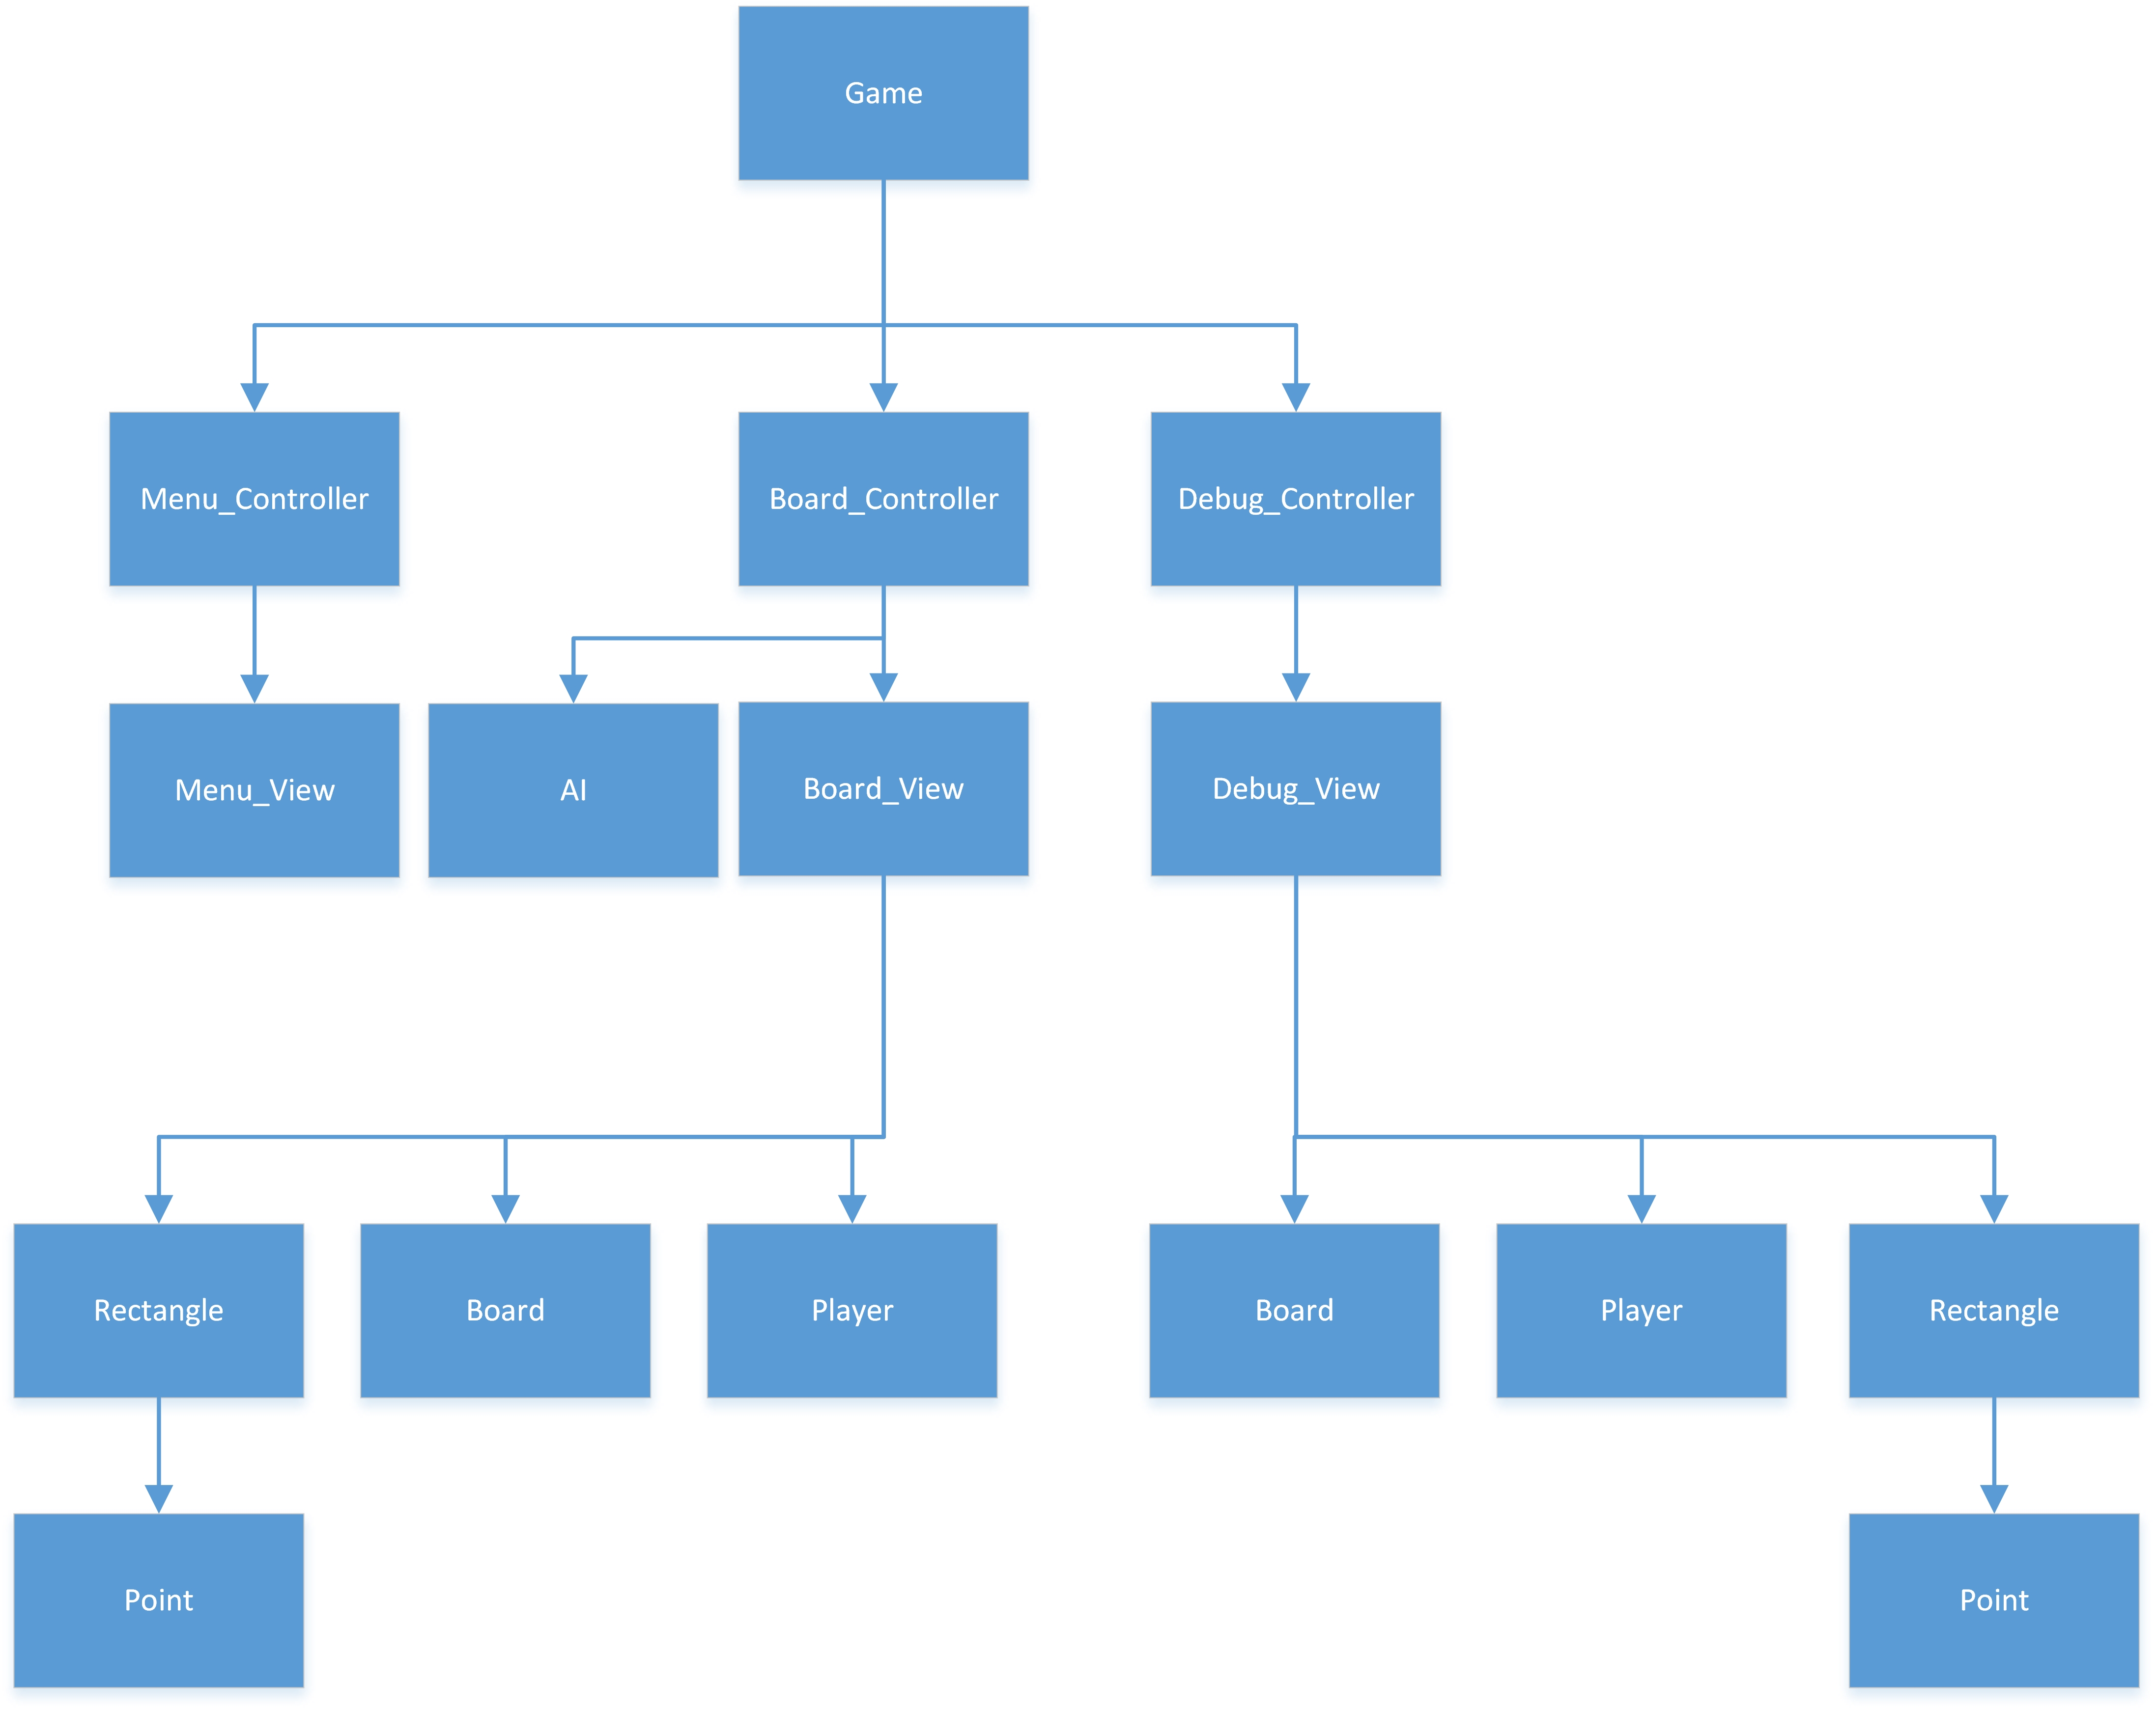
\includegraphics[keepaspectratio=true,scale=0.9]{Uses_Relationship_Tree.jpg}}
  \captionof{figure}{The Decomposition Hierarchy}
\end{minipage}

\section{Anticipated Changes \& Discussion}
In the design of Assignment 1, we anticipated the following changes:
\begin{itemize}
	\item The Board\_Controller can move between different states (i.e. setup, play, results)
	\item The player can play against the computer
	\item The application must efficiently store and search for a piece's next path
	\item There game can be expanded to N Men's Morris, where N is greater than 6
	\item Additional components can be added onto the Board\_View and the Debug\_View
	\item Users can make an infinite number of moves
	\item The platform which to run the game will change over time
	\item The resolution of computer screens will change over time
\end{itemize}

The following subsections will examine each of the items above, and it will discuss how design decisions were made in Assignment 1 in order to accommodate for these changes.

\subsection{There Can Be More States than the Defined States}
The MenuController class allows for additional classes to be added to the application. It serves as a link to other states, so that an unforeseen state, such as the option to play another game besides N-Men’s Morris can be implemented as another module within the same application.

\subsection{The Player Can Play Against the Computer}
In this application, the Player is modelled as an abstract data type. This means that a computer can be programmed to call commands that a human user could make using the mouse. Instead of solely relying on mouse input to place pieces on the board, mouse events trigger methods in the Player object, which in turn places a piece on the board. 

\subsection{The application must efficiently store and search for a piece's next path}
The board in this application is implemented as a 1 dimensional array. This means that every element in the array will contain a value, so that no additional space is required. Also, the board is represented such that the adjacent nodes are beside each other in the array, or eight spots in front or behind. This makes checking the state of the board efficient, as a series of modular functions can be used in order to check the relevant pieces. The use of recursion can be avoided, as the traditional graph representation unused, hence saving both time and space.

\subsection{The Game Can Be Expanded to N Men's Morris}
The modules are implemented such that the number of layers (of rectangles) the board contains, and the number of pieces each player has is contained in variables such as N and NUMBER\_OF\_PIECES. This makes modification of such parameters simple, as the rest of the code will remain constant. 


\subsection{Additional Components Can Be Added to the Views}
Different components of the screen are encapsulated into JPanels which are then assembled in the controller. This allows for new components to be created as JPanels which can then replace existing components in the screen.

\subsection{The Users Can Make an Infinite Number of Moves}
The turn based system is implemented such that one player increments the turn counter while the other player decrements the turn counter. This makes the turn counter switch between 0 and 1. This allows for an infinite number of moves to be played while using as little space as possible. That is, the program will not crash if 2 computers decided to play against each other, and they use more than 2\textsuperscript{32} moves.

\subsection{The Platform Will Change Over Time}
Java was the language of choice because it allowed for cross-platform integration of the application. Additionally, only the standard Java libraries were used in order to allow users to run the application with the minimal number of additional installations. This saves usage space, and it further prevents compatibility and licensing issues. The user of standard Java library is also, in our opinion, the best guarantee that the libraries used will be supported, as long as Java is supported.

\subsection{The Resolution of Computer Screens Will Change Over Time}
The program has been designed to fit screens of all shapes and sizes. The size of the components on the screen is based on the the screen's width and height, and the user can resize the screen so that it fits comfortable on their monitor. The screen is rendered at a resolution of 500 x 500, which is small for 2016 standards, so that it can accommodate platforms with smaller screens, but it can be scaled indefinitely large for larger screens.

\section{Test Plan/Design}
\subsection{Requirement 1: Enable the user to set up a board to play the game}
\begin{table} [h]
	\centering
	\caption{Testing Requirement 1}
    \begin{tabular}{|p{6cm}|p{6cm}|}
        \hline
       	\textbf{Input} & \textbf{Result} \\ \hline
       	Run MenuController and choose Start game. & Window with a board with 2 rectangles, within the other, with circles on the corners and at the midpoint of the lines. Lines connecting the middle circles of the big rectangle to the middle circles of the middle rectangle.  \\
        \hline
    \end{tabular}
\end{table}

Conclusion: This is the proper set-up for 6 Men's Morris.
\newpage
\subsection{Requirement 2: The board includes 2 types of discs}
\begin{table} [h]
	\centering
	\caption{Testing Requirement 2}
    \begin{tabular}{|p{6cm}|p{6cm}|}
        \hline
       	\textbf{Input} & \textbf{Result} \\ \hline
       	Run MenuController, choose start game, place discs on black circles. & Discs placed alternate between red and blue, the first colour determined randomly.  \\
        \hline
    \end{tabular}
\end{table}

Conclusion: There are red and blue discs

\subsection{Requirement 3: The discs are placed on either side of the board}
\begin{table} [h]
	\centering
	\caption{Testing Requirement 3}
    \begin{tabular}{|p{6cm}|p{6cm}|}
        \hline
       	\textbf{Input} & \textbf{Result} \\ \hline
       	Run MenuController, choose start game, place discs on black circles. & On the left there is the amount of Blue discs remaining, on the right the amount of Red (beginning with 6 discs each). When a disc is place the number decreases depending on the colour of the disc placed.  \\
        \hline
    \end{tabular}
\end{table}

Conclusion: The amount of discs for each player is placed on the sides of the board. The amount of discs decreases as they are placed.

\subsection{Requirement 4: There are no discs at the start of the game}

\begin{table} [h]
	\centering
	\caption{Testing Requirement 4}
    \begin{tabular}{|p{6cm}|p{6cm}|}
        \hline
       	\textbf{Input} & \textbf{Result} \\ \hline
       Run MenuController, choose start game. & All the circles on the board are black, not red or blue. \\
        \hline
    \end{tabular}
\end{table}

Conclusion: Black circles mean there are no discs placed on them. There are no discs at the start of the game.

\newpage
\subsection{Requirement 5: The order of play is determined randomly}

\begin{table} [h]
	\centering
	\caption{Testing Requirement 5}
    \begin{tabular}{|p{6cm}|p{6cm}|}
        \hline
       	\textbf{Input} & \textbf{Result} \\ \hline
       Run MenuController, choose Start Game and place a piece anywhere. & Blue piece placed \\ \hline
       Run MenuController, choose Start Game and place a piece anywhere. & Red piece placed \\ \hline
       Run MenuController, choose Start Game and place a piece anywhere. & Blue piece placed \\ \hline
       Run MenuController, choose Start Game and place a piece anywhere. & Blue piece placed \\
        \hline
    \end{tabular}
\end{table}

Conclusion: The starting colour is not consistent; therefore, the starting colour is randomly decided every time.

\subsection{Requirement 6: The user should be able to start a new game, or enter discs to represent the current state of the game}

\begin{table} [h]
	\centering
	\caption{Testing Requirement 6}
    \begin{tabular}{|p{6cm}|p{6cm}|}
        \hline
       	\textbf{Input} & \textbf{Result} \\ \hline
       Run MenuController, click Start Game. & Menu with option of Start game or Debug. When Start game button clicked goes to game mode. \\ \hline
      Run MenuController, click Debug. & Menu with option of Start game or Debug. When Debug chosen it gives the user the option of what  colour to place and user is able to place pieces. \\
        \hline
    \end{tabular}
\end{table}

Conclusion: Menu directs the user to either game mode or to place pieces and then start the game.

\newpage
\subsection{Requirement 7: The user should be able to enter discs to represent the current state of a game by selecting a colour and clicking on the position of the disc}

\begin{table} [h]
	\centering
	\caption{Testing Requirement 7}
    \begin{tabular}{|p{6cm}|p{6cm}|}
        \hline
       	\textbf{Input} & \textbf{Result} \\ \hline
       Run MenuController and choose Debug, choose colours and click circles. & Circles clicked change to the colour of the colour chosen from the menu on the left. \\
        \hline
    \end{tabular}
\end{table}

Conclusion: The circles clicked change to the colour chosen and the user is able to enter the discs to represent a state of the game.


\subsection{Requirement 8: When all discs the user wants to play have been played, the system should analyse whether the current state is possible}

\begin{table} [h]
	\centering
	\caption{Testing Requirement 8}
    \begin{tabular}{|p{6cm}|p{6cm}|}
        \hline
       	\textbf{Input} & \textbf{Result} \\ \hline
       Run MenuController, choose Debug, place 4 blue pieces and 4 red pieces. Play game. & Game mode begins. \\ \hline
       Run MenuController, choose Debug, place 1 blue pieces and 3 red pieces. Play game. & The user receives an error message. \\ \hline
       Run MenuController, choose Debug, place 3 blue pieces and 1 red pieces. Play game. & The user receives an error message. \\ \hline
        Run MenuController, choose Debug, place 10 blue pieces and 3 red pieces. Play game. & The user receives an error message. \\ \hline
      Run MenuController, choose Debug, place 3 blue pieces and 10 red pieces. Play game. & The user receives an error message. \\
        \hline
    \end{tabular}
\end{table}

Conclusion: When a legal amount of discs are placed, the player is able to play the game. When an illegal amount of discs is placed, the user receives an error message.

\newpage
\subsection{Requirement 9: Errors should be displayed to the user}

\begin{table} [h]
	\centering
	\caption{Testing Requirement 9}
    \begin{tabular}{|p{6cm}|p{6cm}|}
        \hline
       	\textbf{Input} & \textbf{Result} \\ \hline
       Run MenuController, choose Debug, place 10 blue pieces and 6 red pieces. Play game. & Error window appears, there are too many pieces. \\ \hline
      Press OK on error message, replace all pieces with black. Play game & Error window appears, both players have fewer than 3 pieces. \\
        \hline
    \end{tabular}
\end{table}

Conclusion: When a user tries to make an impossible state the application tells them that it is illegal and why. The user is able to go back and change the discs to create a legal state.

\section{Conclusion}
This report details the design decisions made and the implementation of assignment 1. Overall, we believe that this is a robust implementation of Six Men's Morris that exemplifies the principles of software engineering. The requirements of this application were first formally defined, and attempts at using tabular expressions and mathematical functions to model the problem were made. This lead to the inception of an board-checking algorithm which allows for the board to have a space complexity  proportional to the number of pieces on the board while maintaining linear search time in the worst case. Furthermore, three separate controllers and views were developed from formally defining the requirements, which allowed each state of the application to remain independent of the other states. This allows our program to exhibit separation of concerns. Through the decomposition of our program, we were able to separate our program into three main areas, models, controllers, and views. This ultimately allowed us to create a program using the MCV architecture. The components of the MCV model in the implementation allowed for modularity and abstraction. ADTs were created which allowed for information hiding, low coupling between different states, and high cohesion. The creation of modules also allowed us to anticipate change. We were able to implement the assignment such that it can be easily modified to accommodate future changes. Both separation of concerns and modularity in our code allow us to implement future changes with minimal change to the overall interface of the code. 

Therefore, since our implementation of assignment 1 embodies all of the principles of software engineering, we believe that our application is a robust implementation of Six Men's Morris.

\end{document}

